\documentclass[12pt]{article}
\usepackage[utf8]{inputenc}
\usepackage[english]{babel}
\usepackage{bbding}
\decimalpoint
\usepackage[spanish]{babel}
\usepackage{amsmath}
\usepackage{amsthm}
\usepackage{amssymb}
\usepackage{graphicx}
\usepackage[margin=0.9in]{geometry}
\usepackage{fancyhdr}
\usepackage[inline]{enumitem}
\usepackage{float}
\usepackage{cancel}
\usepackage{minted}
\usepackage{bigints}
\usepackage{color}
\usepackage{xcolor}
\usepackage{subfig}
\usepackage{listingsutf8}
\usepackage{algorithm}
\usepackage{tocloft}
\usepackage[none]{hyphenat}
\usepackage{graphicx}
\usepackage{grffile}
\usepackage{tabularx}
\usepackage[nottoc,notlot,notlof]{tocbibind}
\usepackage{times}
\usepackage{color}
\definecolor{gray97}{gray}{.97}
\definecolor{gray75}{gray}{.75}
\definecolor{gray45}{gray}{.45}
\renewcommand{\cftsecleader}{\cftdotfill{\cftdotsep}}
\pagestyle{fancy}
\setlength{\headheight}{15pt} 
\lhead{Secret-key primitives}
\rhead{\thepage}
\lfoot{ESCOM-IPN}
\renewcommand{\footrulewidth}{0.5pt}
\setlength{\parskip}{0.5em}
\newcommand{\ve}[1]{\overrightarrow{#1}}
\newcommand{\abs}[1]{\left\lvert #1 \right\lvert}
\date{March 06, 2019}
\title{Session 4: Secret-key primitives}
\author{Session 4}
\usepackage{minted}
\setminted{
    style=emacs,
    breaklines=true
}

%Permite crear columnas en el documento
\usepackage{multicol} 
\usepackage{color}
\usepackage{comment}
\newcommand{\tabitem}{~~\llap{\textbullet}~~}
\newcommand{\subtabitem}{~~~~\llap{\textbullet}~~}

\usepackage{cmbright}                               % Font


\bibliographystyle{IEEEtran}
\begin{document}
		\begin{titlepage}
			\begin{center}
				
				% Upper part of the page. The '~' is needed because \\
				% only works if a paragraph has started.
				
				\noindent
				\begin{minipage}{0.5\textwidth}
					\begin{flushleft} \large
						
\includegraphics[width=0.3\textwidth]{../ipn.png}
					\end{flushleft}
				\end{minipage}%
				\begin{minipage}{0.55\textwidth}
					\begin{flushright} \large
						\includegraphics[width=0.7\textwidth]{../escom.png}
					\end{flushright}
				\end{minipage}
				
				\textsc{\LARGE Instituto Politécnico Nacional}\\[0.5cm]
				
				\textsc{\Large Escuela Superior de Cómputo}\\[1cm]
				
				% Title
				
				{ \huge Session 4: Secret-key primitives \\[1cm] }
				
				{ \Large Cryptography} \\[1cm]
				
				{ \Large Group: 3CM6 } \\[1cm]
				
				\noindent
				\begin{minipage}{0.5\textwidth}
					\begin{flushleft} \large
						\emph{Students:}\\
						
						\begin{tabular}{ll}
					     Nicolás Sayago Abigail\\
					     Naranjo Ferrara Guillermo\\
					     
					\end{tabular}
					\end{flushleft}
				\end{minipage}%
				\begin{minipage}{0.5\textwidth}
					\begin{flushright} \large
						\emph{Teacher:} \\
						Díaz Santiago Sandra  \\
					\end{flushright}
				\end{minipage}
				
				\vfill
				
				% Bottom of the page
				{\large March 06, 2019}
			\end{center}
		\end{titlepage}
	
	\tableofcontents
	\newpage
	
	% ------------------------------------------------------------------------
	%                                    INSTRUCTIONS
	% ------------------------------------------------------------------------
	\section{Instructions}
        In this session we will work with primitives for symmetric cryptography.
        \begin{enumerate}
            \item Choose two different cryptographic libraries, consider your favorite programming language and find wich are the blockciphers, stream ciphers, modes of operation and cryptographically secure pseudorandom bit generators, that are included in the library.
            
            \item Choose the web site of a bank or a web site to make online shopping, gind information about the ecryption algorithms the web site uses to protect their communicatins. List the algorithms and find what is the meaning of the acronym for each cryptographic mechanism. Determine which of them are symmetric and which of them are asymmetric.
        \end{enumerate}
	
	% ------------------------------------------------------------------------
	%                                    TOPICS
	% ------------------------------------------------------------------------
	\section{Topic}
	    \subsection{Symmetric encryption}
	        Also referred to as conventional encryption or single-key encryption, was the only type of encryption in use prior to the development of public-key encryption in the 1970s.
	        
	        \begin{center}
                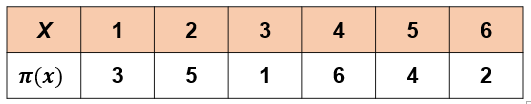
\includegraphics[width=0.9\textwidth]{Practica4/images/T1.PNG}
            \end{center}
	
	    \subsection{Block ciphers}
	        A block cipher is one in which a block of plaintext is treated as a whole and used to produce a ciphertext block of equal length. Typically,  a block size of 64 or 128 bits is used. As with a stream cipher, the two users share a symmetric encryption key. Using some of the modes of operation, a block cipher can be used to achieve the same effect as a stream cipher. 
	        
	        In general, they seem applicable to a broader range of applications than stream cipher. The vast majority of network-based symmetric cryptographic applications make use of block ciphers.
	   
	        \begin{center}
                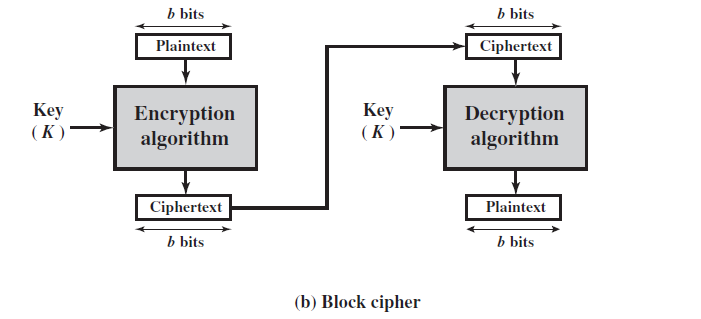
\includegraphics[width=0.9\textwidth]{Practica4/images/blockcipher.PNG}
            \end{center}
            
	    \subsection{Stream ciphers}
	        A stream cipher is one that encrypts a digital data stream one bit or one byte at tyme. Examples of classical stream ciphers are the aukeyed Vinegere cipher and the Vernam cipher. 
	        
	    \subsection{Modes of operation}
	    
	    \subsection{Cryptographically secure pseudorandom bit generators}
	    
	% ------------------------------------------------------------------------
	%                               EXERCISE 1
	% ------------------------------------------------------------------------
	\section{Exercise 1}
	
	    \subsection{Programming lenguage C++}
	        % ---------------------------------------------------------
    	    %                          C++
    	    % ---------------------------------------------------------

	        \begin{itemize}
	            \item[\checkmark] \textbf{Blockciphers}     \\
	                % AQUI PONER INVESTIGACION
	                
	            \item[\checkmark] \textbf{Stream ciphers}   \\
                    % AQUI

	            \item[\checkmark] \textbf{Modes of operation}   \\
                
                \item[\checkmark] \textbf{Cryptographically secure pseudorandom bit generators}   \\

	        \end{itemize}
	    % ---------------------------------------------------------
	    %                      JAVASCRIPT
	    % ---------------------------------------------------------
	    \subsection{Programming lenguage JAVASCRIPT}
	        \begin{itemize}
	            \item[\checkmark] \textbf{Blockciphers}     \\
	                % AQUI PONER INVESTIGACION
	                
	            \item[\checkmark] \textbf{Stream ciphers}   \\
                    % AQUI

	            \item[\checkmark] \textbf{Modes of operation}   \\
                
                \item[\checkmark] \textbf{Cryptographically secure pseudorandom bit generators}   \\

	        \end{itemize}
	    
	% ------------------------------------------------------------------------
	%                               EXERCISE 2
	% ------------------------------------------------------------------------
	\section{Exercise 2}
	
	
	
	
        	
 \end{document}